\documentclass[11pt]{article}
\usepackage{geometry}                % See geometry.pdf to learn the layout options. There are lots.
\geometry{letterpaper}                   % ... or a4paper or a5paper or ... 
%\geometry{landscape}                % Activate for for rotated page geometry
%\usepackage[parfill]{parskip}    % Activate to begin paragraphs with an empty line rather than an indent
\usepackage{graphicx}
\usepackage{amsmath}
\usepackage{amssymb}
\usepackage{epstopdf}
\usepackage{hyperref}
\DeclareGraphicsRule{.tif}{png}{.png}{`convert #1 `dirname #1`/`basename #1 .tif`.png}

\newtheorem{claim}{Claim}

\title{Hierarchical iPOMDPs for HRL}
\author{Momchil}
%\date{Nov 2, 2017}                                           % Activate to display a given date or no date

\begin{document}
\maketitle
%\section{}
%\subsection{}






\section{Background} 

Define MDPs, RL framework
POMDPs
Multi-task RL
HRL = sMDPs
Option discovery as hidden state inference
POMDP formulation for one environment
Multi-task POMDP

\subsection{Reinforcement Learning and Markov Decision Processes}

In reinforcement learning (RL), tasks are traditionally represented as Markov decision processes (MDPs) \cite{Sutton1998} and we will use those two terms interchangably. We define an MDP as a tuple $(\mathcal{S}, \mathcal{A}, T, R, I, \mathcal{F})$ where:
\begin{itemize}
\item $\mathcal{S}$ is a set of states that the agent can occupy,
\item $\mathcal{A}$ is a set of actions that the agent can perform in those states,
\item $T(\cdot|s,a)$ is a distribution of next states, such that $T(s'|s,a)$ is the probability that the agent ends up in state $s' \in \mathcal{S}$ after executing action $a \in \mathcal{A}$ in state $s \mathcal{S}$,
\item $R(s,a)$ is the amount of reward an agent obtains after executing action $a$ in state $s$,
\item $I(\cdot)$ is a distribution of initial states in which the agent may start the task,
\item $\mathcal{F}$ is a set of terminal states in which the task is completed.
\end{itemize}

The agent begins the task in state $s_0 \sim I$. At each time step $t$, the agent performs action $a_t$ that takes it from state $s_t$ to state $s_{t+1} \sim T(\cdot|s_t,a_t)$ and receives reward $r_t \sim R(s_t, a_t)$. The agent is said to follow a policy $\pi$ if it chooses its actions according to $a_t \sim \pi(\cdot|s_t)$.

For a fixed policy $\pi$, the state-value function $V_\pi(s)$ represents the total expected discounted reward for each state $s$. It is the sum of all future rewards that the agent will receive, on average, if it starts in state $s$ and follows $\pi$:

\[
V_{\pi}(s) = \mathbb{E}_{\pi} \left[  \sum_{t=0}^{\infty} \gamma^{t} r_t \middle| s_0 = s \right] ,
\]

where $\gamma$ is the discount rate which determines the present value of future rewards. The goal of the agent is to select an optimal policy $\pi^*$ that maximizes $V_{\pi^*}(s)$. The optimal value function $V_{\pi^*}(s)$ satisfies the Bellman optimality equation \cite{Bellman1957}:

\begin{align*}
V_{\pi^*}(s) = \max_a  \left\{ R(s,a) + \gamma \sum_{s'} V_{\pi^*}(s') \,\, T(s'|s,a) \right\} 
\end{align*}

The Bellman equation serves as a basis of a number of algorithms for solving optimal control problems.

\subsubsection{RL in the Brain}

RL algorithms often fall into one of two broad categories: model-free algorithms, in which the agent learns $V_\pi$ directly; and model-based algorithms, in which the agent learns $R$ and $T$ to compute $V_\pi$.  Computational cognitive neuroscience has borrowed this dichotomy as a formal description of the distinction between habitual and goal-directed behaviors \cite{Dolan2013}. Model-free accounts of habitual behaviors posit that animals learn automatic responses to stimuli if they tend to lead to rewarding outcomes. Model-based accounts of goal-directed behaviors posit that animals learn the statistics of the environment independently of the rewards.

Model-free accounts are less computationally intensive, however they require many training examples and have to be re-trained whenever the reward distribution changes. This is consistent with empirical observations that overtrained animals exhibit fast reaction times and rigid behavioral patterns that tend to persist even reward contingencies change. Model-free accounts are further bolstered by the hallmark discovery that the phasic firing of midbrain dopaminergic neurons closely tracks the model-free reward prediction error (RPE) signal.

Model-based accounts, on the other hand, predict that agents will flexibly adapt to changes in reward distributions, at the cost of slower reaction times due to the greater computational complexity. Model-based accounts explain phenomena such as latent learning and accord with the intuition that people don't have to learn a new policy, say, every time they go shopping for different groceries.

\subsection{Hierarchical Reinforcement Learning and Semi-Markov Decision Processes}

A long-standing challenge for traditional RL is the combinatorial explosion that occurs when planning and learning take place over long time horizons. This challenge been addressed by hierarchical reinforcement learning (HRL), which breaks down the problem into sub-problems at multiple levels of abstraction.

One strand of HRL extends the agent's action repertoire to include \textit{options} \cite{Sutton1999} -- temporally-extended sequences of actions, sometimes referred to as subroutines, partial policies, or macro-actions. Each option consists of a sequence of actions that are executed as a single behavioral unit. Actions in the original MDP are referred to as \textit{primitive actions}, in order to distinguish them from options.

Formally, including options turns the underlying MDP into a discrete-time semi-Markov decision process (SMDP), which allows transitions between states to take variable amounts of time. Thus we augment the original MDP with the following definitions:

\begin{itemize}
\item $\mathcal{O}$ is a set of options,
\item $\pi_o$ is a policy for each option $o \in \mathcal{O}$, such that while $o$ is being executed, actions are selected according to $a \sim \pi_o(\cdot|s)$,
\item $\mathcal{F}_o$ is a set of subgoal states for each option $o$, such that $\pi_o$ terminates when reaching any one of those states,
\item $T(\cdot,\cdot|s,o)$ is a joint distribution of terminal states and step counts for each option $o$, such that $T(s',t|s,o)$ is the probability that the agent ends up in subgoal state $s' \in \mathcal{F}_o$ exactly $t$ time steps after executing option $o \in \mathcal{O}$ in state $s \in \mathcal{S}$,
\item $R(s,o)$ is the total expected discounted reward for starting in state $s$ and executing option $o$.
\end{itemize}

The rewards can be computed as:

\begin{align*}
R(s,o) = \mathbb{E} \left[ \sum_{t=0}^\infty \gamma^t r_t \middle| s_0 = s, a_t \sim \pi_o \right]
\end{align*}

It is also convenient to define a discounted distribution of terminal states \cite{Sutton1999}:

\begin{align*}
T_\gamma(s'|s,o) = \sum_{t=0}^\infty T(s',t|s,a) \gamma^t
\end{align*}

In the SMDP, the agent follows a policy $\mu$ defined over options, such that options are chosen according to $o_t \sim \mu(\cdot|s_t)$. The Bellman equation for the optimal options policy $\mu^*$ thus becomes:

\begin{align*}
V_{\mu^*}(s) = \max_o  \left\{ R(s,o) + \sum_{s'} V_{\mu^*}(s') \,\, T_\gamma(s'|s,o) \right\} 
\end{align*}

An options policy $\mu$ in the SMDP uniquely determines a \textit{flat policy} $\pi$ consisting solely of primitive actions in the original MDP. Thus any solution of the SMDP can be mapped back to a solution in the original MDP.

Introducing options allows agent to perform ``jumps'' in the state space. When considering an option $o$, the agent only needs to compute the value of its subgoal states $s' \in \mathcal{F}_o$, without computing the values of intermediate states that will be traversed while executing the option. If the subgoals and the options policies are chosen appropriately, exploration and planning can be performed much more efficiently by allowing the agent reason over short sequences of options, rather than over long sequences of primitive actions.

\subsubsection{HRL in the Brain}

In addition to its computational benefits, HRL provides an appealing account of habitual behaviors \cite{Botvinick2008} that competes with model-free RL. Model-free RL fails to capture habits which unfold as sequences of actions in response to a single cue, disregarding intervening cues \cite{Dezfouli2013}. It also fails to specify how habitual responses can be generalized across multiple task contexts.

Options as defined in HRL map nicely to habitual action sequences and their neural substrates. Research on rodents has implicated striatal and midbrain neurons in the formation and initiation of habitual action sequences, with task-bracketing activity emerging over the course of training in both regions \cite{Smith2013, Jin2014}. In these tasks, ``bumps'' of neural activity emerge at key decision points during the trial (e.g., at the trial start or at maze junctions), while activity is generally low in the remainder of the trial (e.g., while running straight). Similar task-bracketing activity has also been observed in birds and primates, suggesting a conserved neural implementation \cite{Smith2013}. The acquisition, initiation and termination of options in HRL may account for these diverse findings.

Additionally, the HRL framework has been directly supported by both behavioral \cite{Botvinick2014} and neural evidence \cite{Ribas-Fernandes2011}. It is also consistent with our intuition that people can plan over different time scales (e.g., go shopping, pick up the kids, etc.) without being bogged down by the details (e.g., get up, turn left, step forward, etc.).


\subsection{Option Discovery and Transfer}

The traditional HRL does not specify how options are transferred across tasks. Intuitively, under some circumstances, transferring an option from a previous task would speed up learning on a novel task (for example, learning to make a cup of coffee after learning to make a cup of tea). In other instances, learning a new task might be inhibited by previously acquired options, such as the tendency to get stuck in pre-existing ways of thinking that preclude creative solutions to new problems, a phenomenon known as the Einstellung effect \cite{Bilalic2008}. HRL does not make it clear why an agent faced with a new task would choose to execute an option acquired in a previous task, particularly if the state space of the new task is different. The problem of transferring behaviors from a source task to a target task has been investigated in the field of transfer learning and is often solved via an explicit inter-task mapping between states in the two tasks \cite{Taylor2009}. This mapping is often supplied manually or is discovered offline via batch heuristic methods which lack biological plausibility.

Furthermore, HRL fails to specify how options are learned in the first place, with most HRL accounts assuming a pre-specified set of options \cite{Botvinick2008}. The problem of discovering useful options has traditionally been addressed in an ad-hoc fashion, often by breaking down a task into multiple sub-tasks and defining the optimal solution to each sub-task as a separate option. The sub-tasks are often defined either by manually designating certain states as subgoal states using internal rewards (``pseudo-rewards''), or by partitioning the original task space based on the topology of the state transition structure (for example, by identifying ``bottleneck'' states such as doorways, or clusters of interconnected states such as rooms) \cite{Botvinick2008}. Solway et al. \cite{Solway2014} proposed a more principled solution based on Bayesian model selection. In their study, they showed that useful options can be learned by considering an ensemble of tasks occurring in the same environment. Human behavior was consistent with a decomposition of the environment into sub-tasks, each solved by a corresponding option, such that the resulting task hierarchy yields the most parsimonious explanation of optimal behaviors in the full task ensemble.

Even though it is limited by strong assumptions about the state space and the transition dynamics, the approach of Solway et al. highlights the importance of explicitly considering a distribution of tasks. In fact, most heuristic approaches to option discovery implicitly assume a task distribution, often by assuming that each accessible state has equal probability of being the start state or the goal state. To illustrate why option discovery only makes sense in the context of ensembles of tasks, consider what would happen if the agent only ever faced a single task in the world: it could then just learn the optimal policy for that one task using regular RL. Options in the HRL sense would thus be unnecessary as the entire policy would be executed automatically, like a single option. Options thus imply a world with multiple tasks. However, if those tasks were completely unrelated, options would again not make sense as the agent would have to learn a separate policy for each task from scratch, much like in the single-task scenario. In order for the agent to be able to learn useful options that can be transferred across tasks, there must be a shared structure between those tasks. While this point may seem trivial, we believe it lies at the crux of understanding how people and animals acquire their rich repertoire of habitual behaviors.

In order to understand how options are learned and facilitate performance on novel tasks, it is therefore necessary to define a probability distribution over tasks in the environment. Crucially, this distribution of tasks would be highly structured \cite{Botvinick2015}, such that tasks are grouped into families of tasks that share certain parameters which are not directly observable. Hierarchy discovery would thus correspond to a particular kind of hidden state inference, where the hidden state refers to the parameters that govern the distribution of tasks.

\subsection{Multi-task Reinforcement Learning}

\begin{figure}
\centering
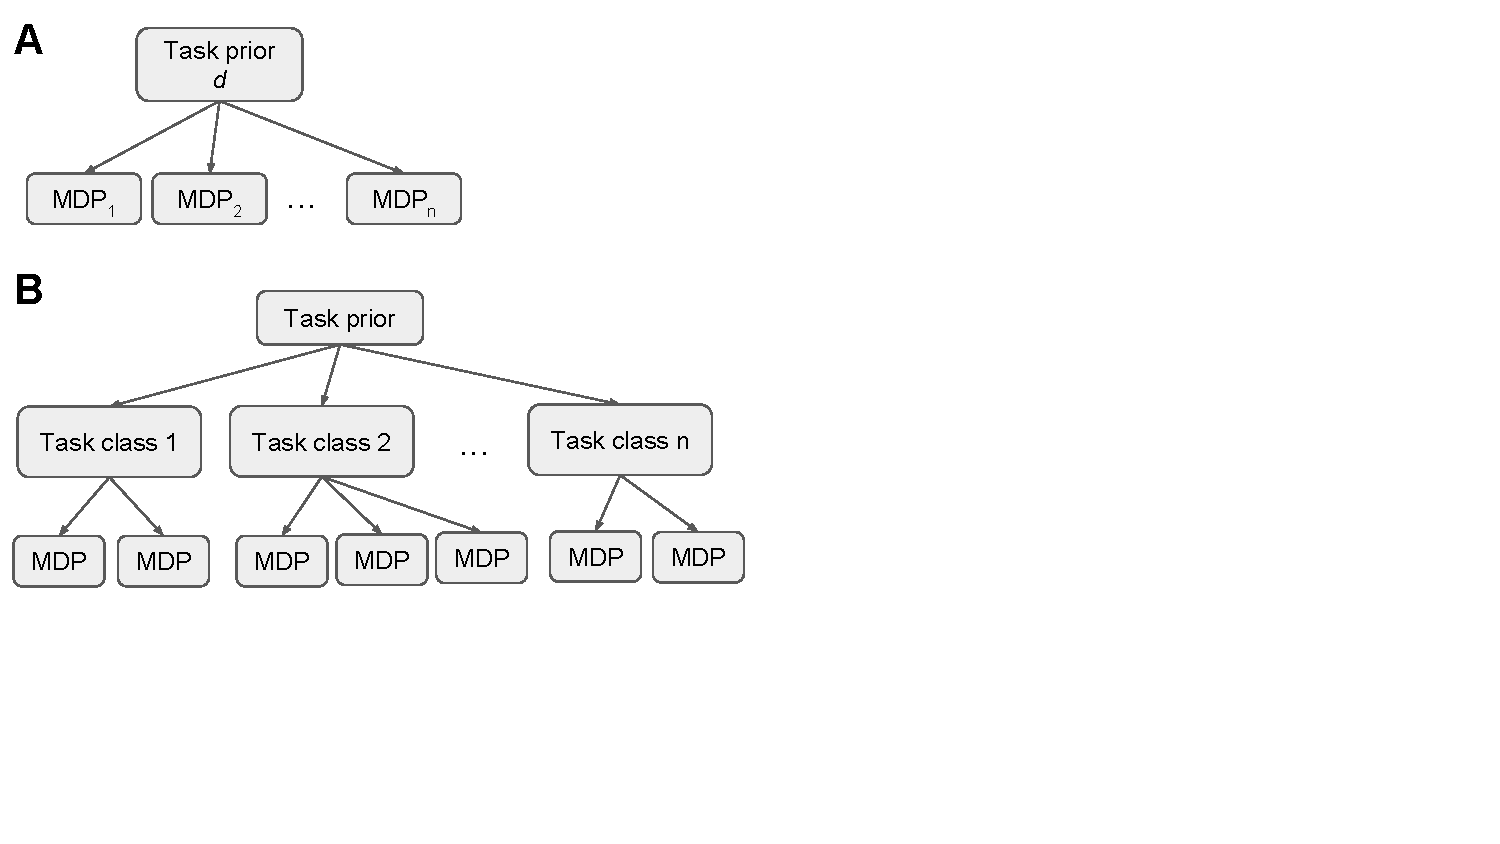
\includegraphics[scale=0.7,  trim = 0 120 400 10]{figures/wilson.pdf}
\caption{(A) The MTRL framework, (B) MTRL with classes of tasks. Adapted from \cite{Wilson2007}.}
\label{fig:mtrl}
\end{figure}

The problem of optimizing behaviors for a set of tasks (MDPs) drawn from a common distribution is the focus of multi-task reinforcement learning (MTRL) \cite{Wilson2007}. In MTRL, MDPs are assumed to be drawn from the same prior distribution. Experiencing a sequence of MDPs can allow the agent to infer the hidden parameters of the distribution and to quickly discover the optimal policy for a new MDP drawn from the same distribution.

Wilson et al. \cite{Wilson2007} extended this framework to include \textit{classes} of tasks, where each class defines its own distribution of MDPs (Figure~\ref{fig:mtrl}). Their model allows the agent to rapidly discover the structure of tasks similar to previous tasks, while simultaneously supporting the discovery of entirely new classes of tasks. Policies acquired in old tasks can thus be adapted to new tasks from the same class.

\subsubsection{MTRL for HRL}

While Wilson et al.'s approach beings to address the question of policy transfer across MDPs, it leaves open several questions:

\begin{itemize}
\item How does ambiguity between MDPs arise? Traditional tabular MDPs assume that the agent is fully aware of what state it is in, which implies it is also fully aware of which MDP it is in. In order to be able to perform inference over MDPs, it must be the case that states are in some sense ``shared'' across MDPs, or at least ``look similar''.
\item What are the distributions over MDPs? Intuitively, they should be generic enough to capture a wide variety of tasks that agents may encounter in the world, while being constrained enough to facilitate efficient learning and generalization.
\item Why would options arise? In order to be able to define useful options and convert a given MDP into an SMDP, there must be some form of modular or subtask structure build into the MDP.
\item Why would options be transferred? In order to transfer options, the modules or subtasks need to be shared across MDPs.
\end{itemize}

We address the first question by appealing to the formalism of partially observable Markov decision processes (POMDPs), in which states are not directly observable but instead define distributions over observations. The agent must thus infer which state it is in based on these observations. In MTRL with POMDPs \cite{Li2009}, the agent additionally infers which POMDP it is in.

We address the second question using infinite POMDPs (iPOMDPs) \cite{DoshiVelez2009}, which allow the agent to flexibly adapt to environments with different state spaces.

We address the third question by constraining the iPOMDPs to a particular modular structure, such that states are grouped into \textit{communities} of states. This is a novel contribution of our work.

We address the last question by allowing the structure and properties of these communities to be shared across different iPOMDPs.






\begin{align*}
\bar{T} \sim \text{GEM}(...) \\
T(.|s) = T_s \sim \text{DP}(..., \bar{T}) \\
\phi_s \sim H \\
s_t \sim T_{s_{t-1}} \\
o_t \sim F(\phi_{s_t})
\end{align*}


\subsection{hierarchical iHMM as HDP}


\begin{align*}
\beta \sim \text{GEM}(...) \\
z_s \sim \text{Mult}(\beta) \\
\bar{T} \sim \text{GEM}(...) \\
\bar{T}_c \sim \text{DP}(..., \bar{T}) \\
T(.|s) = T_s \sim \text{DP}(..., \bar{T}_{z_s}) \\
\phi_s \sim H \\
s_t \sim T_{s_{t-1}} \\
o_t \sim F(\phi_{s_t})
\end{align*}


\begin{align*}
H_c \sim ... \\
\phi_s \sim H_{z_s}
\end{align*}


\subsection{hierarchical iHMM as HDP, version 2}



\begin{align*}
\bar{T} \sim \text{GEM}(...) \\
T(.|c) = T_c \sim \text{DP}(..., \bar{T}) \\
\bar{T}_{c,\cdot} \sim \text{GEM}(...) \\
T(. \in c | s \in c) = T_{c,s} \sim \text{DP}(..., \bar{T}_{c,\cdot}) \\
T_s(s') = T(s'|s) = \begin{cases}  T_{c,s}(s') \,\, T_c(c) & \text{ if } s, s' \in c \\  \bar{T}_{c',\cdot}(s') \,\, T_c(c') & \text{ if } s \in c, s' \in c'  \end{cases} \\
\phi_s \sim H \\
s_t \sim T_{s_{t-1}} \\
o_t \sim F(\phi_{s_t})
\end{align*}


\subsection{hierarchical iHMM as HDP, version 3}



\begin{align*}
\beta \sim \text{GEM}(...) \\
z_c \sim \text{Mult}(\beta) \\
\bar{T}_{g,\cdot} \sim \text{GEM}(...) \\
T_{g,s} \sim \text{DP}(..., \bar{T}_{g,\cdot}) \\
\bar{T} \sim \text{GEM}(...) \\
T(.|c) = T_c \sim \text{DP}(..., \bar{T}) \\
\bar{T}_{c,\cdot} = \bar{T}_{g=z_c,\cdot} \\
T(. \in c | s \in c) = T_{c,s} = T_{g=z_c,s}\\
T_s(s') = T(s'|s) = \begin{cases}  T_{c,s}(s') \,\, T_c(c) & \text{ if } s, s' \in c \\  \bar{T}_{c',\cdot}(s') \,\, T_c(c') & \text{ if } s \in c, s' \in c'  \end{cases} \\
\phi_s \sim H \\
s_t \sim T_{s_{t-1}} \\
o_t \sim F(\phi_{s_t})
\end{align*}


\bibliographystyle{unsrt}
\renewcommand{\refname}{Bibliography \& References Cited}
\bibliography{ihmm_stuff.bib}




\end{document}  